\documentclass[11pt]{article}
\usepackage[utf8]{inputenc}
\usepackage[T1]{fontenc}
\usepackage{lmodern}
\usepackage[letterpaper,margin=2.2cm]{geometry}
\usepackage{graphicx}
\usepackage{booktabs}
\usepackage{array}
\usepackage{longtable}
\usepackage{float}
\usepackage{xcolor}
\usepackage{hyperref}
\usepackage{amsmath}
\hypersetup{colorlinks=true,linkcolor=blue!55!black,urlcolor=blue!65!black,citecolor=teal!55!black}
\graphicspath{{../outputs/figures/}}
\definecolor{navy}{HTML}{102A43}
\definecolor{teal}{HTML}{0F9D91}
\definecolor{soft}{HTML}{F1F5F9}
\newcommand{\repo}{\href{https://github.com/DanielBarillasM/Laboratorio-6.-Analitica-de-Redes-Sociales_Grupo-1_DS_Sec-10}{Repositorio de GitHub}}
\setlength{\parindent}{0pt}
\setlength{\parskip}{0.6em}

\begin{document}

\begin{titlepage}
\pagecolor{navy}\color{white}
\centering
\vspace*{1.4cm}
{\Large Universidad del Valle de Guatemala\par}
\vspace{0.4cm}
{\large Facultad de Ingeniería\par}
{\large CC3084 -- Data Science, Sección 10\par}
\vfill
{\Huge\bfseries Laboratorio 6\par}
\vspace{0.3cm}
{\LARGE Analítica de Redes Sociales\par}
\vspace{0.9cm}
{\Large\color{teal!25!white}Avance reproducible -- 75\%\par}
\vfill
{\large Grupo 1\par}
\vspace{0.5cm}
\begin{tabular}{rl}
Jorge Gabriel Palacios Sales & 231385\\
Pablo Daniel Barillas Moreno & 22193\\
Roberto Emiliano Otoniel & 23968\\
\end{tabular}
\vfill
{\large Segundo semestre de 2026\par}
\end{titlepage}
\nopagecolor\color{black}

\tableofcontents
\newpage

\section{Resumen ejecutivo}

Se analizaron 293 videos, 97 canales, 406 comentarios y 332 autores de una muestra obtenida de YouTube. El avance implementa un flujo reproducible para cargar archivos CSV o Excel, normalizar identificadores, limpiar texto en español, integrar las dos tablas, describir participación y construir redes autor--video. También genera las proyecciones autor--autor y video--video, calcula métricas topológicas y detecta comunidades mediante Louvain ponderado.

El 100\% de los comentarios se asoció con un video. La participación está fuertemente concentrada: el video \emph{Qué rico come tu diputado} contiene 161 comentarios (39.7\% del total), los cinco videos principales reúnen 75.4\%, y el canal Quorum concentra 256 comentarios (63.1\%). La red bipartita completa contiene 625 nodos y 343 aristas; conserva 274 videos aislados para representar la cobertura real. La proyección de autores presenta una componente principal con 83.1\% de los autores y diez comunidades con modularidad 0.395.

El avance cubre 74 de 100 puntos trazables de la rúbrica. La centralidad avanzada, el sentimiento formal en español, el análisis de nodos articuladores y la síntesis final se reservan para la siguiente entrega.

\section{Alcance del avance}

El PDF define como avance mínimo los ejercicios 1 al 4. Para aproximarse al 75\% solicitado se completaron además las proyecciones, la topología y la detección de comunidades. La caracterización temática de comunidades está incluida; su dimensión de sentimiento queda pendiente para emplear una herramienta validada para español.

\begin{table}[H]
\centering
\caption{Cobertura planificada de la rúbrica.}
\begin{tabular}{p{0.53\textwidth}rrl}
\toprule
Criterio & Total & Cubierto & Estado\\
\midrule
Calidad, limpieza y preprocesamiento & 18 & 18 & Completo\\
Análisis exploratorio & 18 & 18 & Completo\\
Red bipartita autor--video & 10 & 10 & Completo\\
Proyecciones & 8 & 8 & Completo\\
Topología y fragmentación & 12 & 12 & Completo\\
Comunidades & 10 & 8 & Falta sentimiento\\
Centralidad y participantes puente & 7 & 0 & Fase final\\
Contenido y sentimiento & 5 & 0 & Fase final\\
Interpretación y conclusiones finales & 12 & 0 & Fase final\\
\midrule
Total & 100 & 74 & Avance aproximado 75\%\\
\bottomrule
\end{tabular}
\end{table}

\section{Datos, unidades e integración}

Cada fila de videos representa un video y su llave primaria es \texttt{video\_id}; cada fila de comentarios representa un comentario principal y su llave es \texttt{comment\_id}. \texttt{channel\_id} identifica el canal propietario, mientras \texttt{author\_channel\_id} identifica al autor del comentario. Los nombres y handles se usan únicamente como etiquetas visibles.

Se utilizaron los archivos originales \texttt{youtube\_videos.csv} y \texttt{youtube\_comments.csv} solicitados por la guía. Ambos fueron verificados como CSV reales. Los 293 identificadores de video están completos y son únicos, por lo que no fue necesario reconstruirlos. El cargador conserva detección por firma binaria y recuperación auditable desde \texttt{video\_url} como controles defensivos ante futuras exportaciones en Excel.

\begin{table}[H]
\centering
\caption{Dimensiones e integración.}
\begin{tabular}{lr}
\toprule
Indicador & Valor\\
\midrule
Videos & 293\\
Canales únicos & 97\\
Comentarios & 406\\
Autores únicos & 332\\
Videos con comentarios & 19\\
Videos sin comentarios & 274\\
IDs de video recuperados & 0\\
Comentarios asociados & 406 (100\%)\\
\bottomrule
\end{tabular}
\end{table}

La relación canal--video es de uno a muchos en la muestra. Un autor puede comentar varios videos y un video puede recibir comentarios de varios autores. \texttt{source\_query} describe cómo se obtuvo el registro, no necesariamente su tema definitivo.

\section{Calidad, limpieza y preprocesamiento}

Se evaluaron dimensiones, tipos, valores faltantes, duplicados, constantes, atípicos y consistencia de IDs, nombres y handles. No hay duplicados completos y las llaves primarias son completas y únicas. \texttt{viewer\_rating} está vacío en los 406 comentarios y \texttt{is\_pinned} es constante; el primero se excluye y el segundo se conserva solo para auditoría. Las fechas relativas no se transforman en fechas exactas.

Los espacios de \texttt{like\_count\_text} se interpretan como cero y el parser contempla separadores y sufijos K, M, \emph{mil} y \emph{millones}. \texttt{reply\_count} se conserva como conteo descriptivo: no identifica autores de respuesta y, por tanto, nunca origina aristas entre usuarios.

Para cada comentario se conserva \texttt{texto\_original} y se produce \texttt{texto\_limpio}. La limpieza decodifica HTML, convierte a minúsculas, elimina URL y menciones, retiene la palabra de los hashtags sin el símbolo, extrae palabras Unicode, elimina números, puntuación, emojis y una lista explícita de stopwords en español. Los emojis permanecen en el original para el futuro análisis de sentimiento. No se aplicó lematización en esta fase porque hacerlo sin un modelo morfosintáctico validado para español podría deformar nombres y términos temáticos.

\begin{table}[H]
\centering
\caption{Efecto cuantificado de la limpieza textual.}
\begin{tabular}{lr}
\toprule
Métrica & Valor\\
\midrule
Registros de entrada & 406\\
Textos modificados & 403\\
Textos vacíos antes & 0\\
Textos vacíos después & 6\\
Duplicados textuales antes & 2\\
Duplicados textuales después & 11\\
Registros eliminados & 0\\
\bottomrule
\end{tabular}
\end{table}

Los textos vacíos posteriores no se eliminan: mantienen la trazabilidad del comentario y sus atributos de red, pero se excluyen naturalmente de frecuencias léxicas.

\section{Análisis exploratorio}

\begin{figure}[H]
\centering
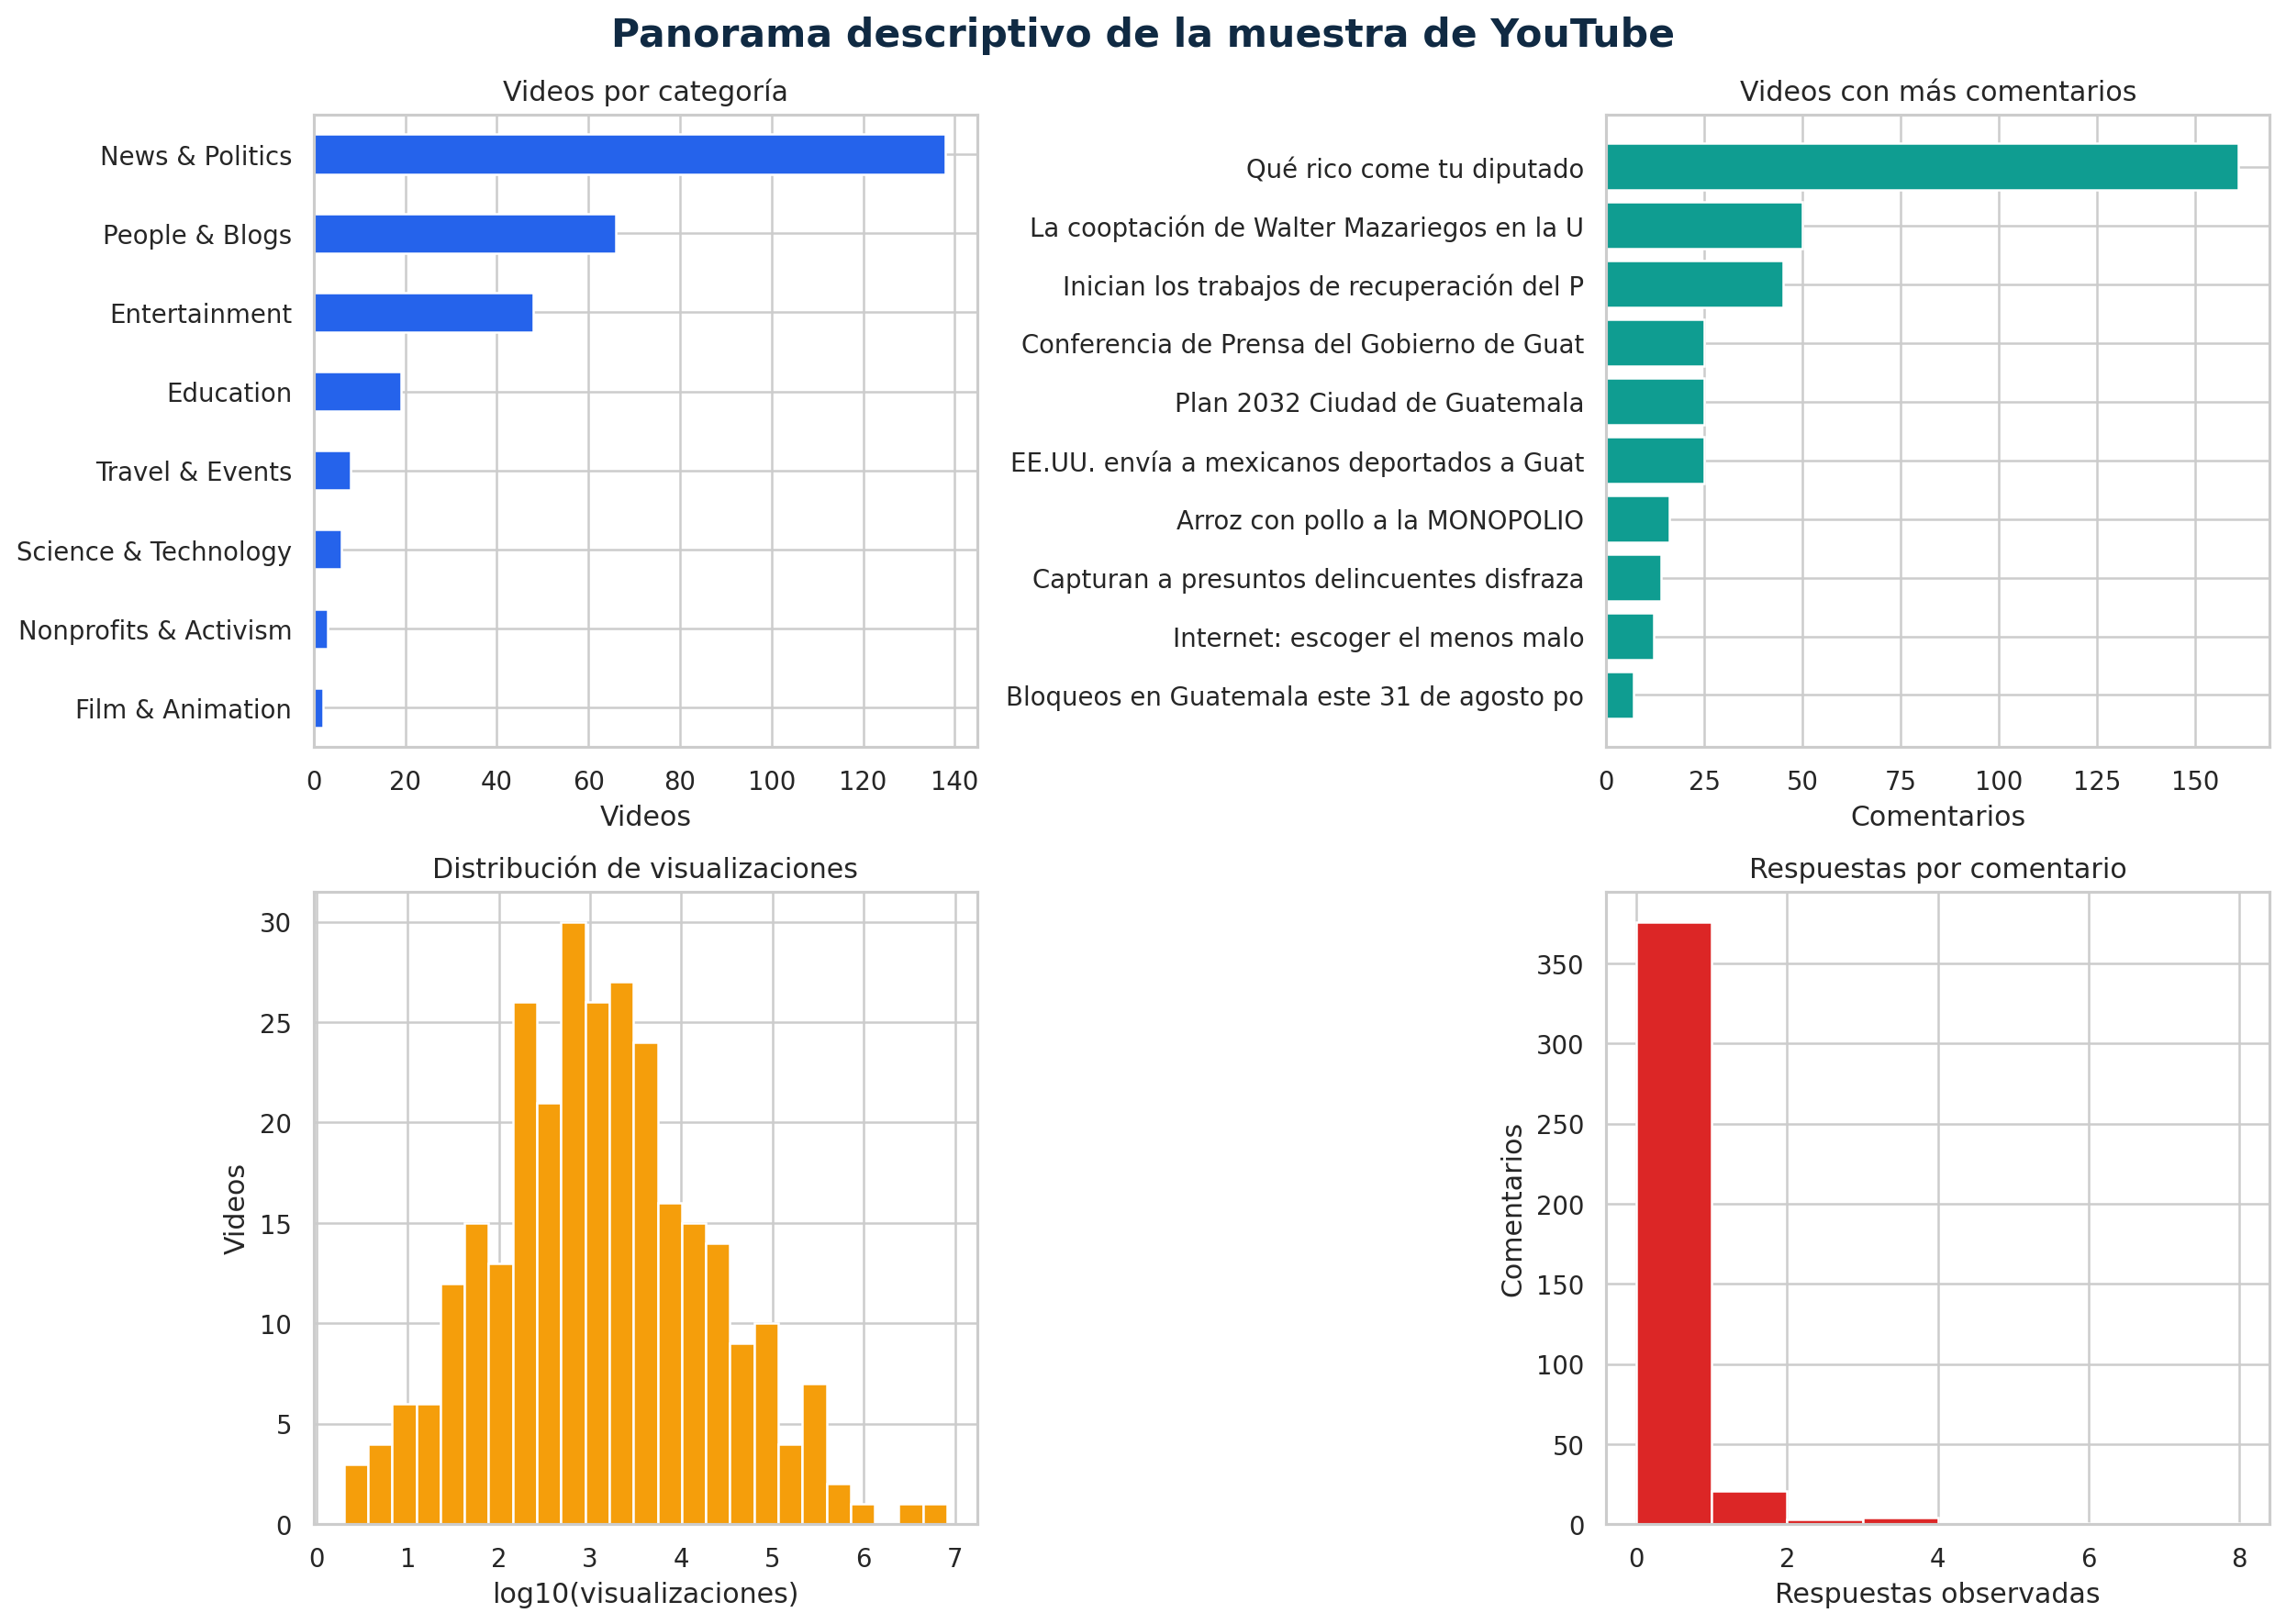
\includegraphics[width=0.98\textwidth]{eda_panorama.png}
\caption{Categorías, participación, visualizaciones y respuestas en la muestra.}
\label{fig:eda}
\end{figure}

La categoría dominante es \emph{News \& Politics}. Las visualizaciones son marcadamente asimétricas: la mediana es 1,175, mientras el máximo supera 8.19 millones. Esta diferencia justifica escalas logarítmicas y medidas robustas. La mayoría de comentarios no recibió respuestas y la cobertura se concentra en solo 19 videos.

\begin{figure}[H]
\centering
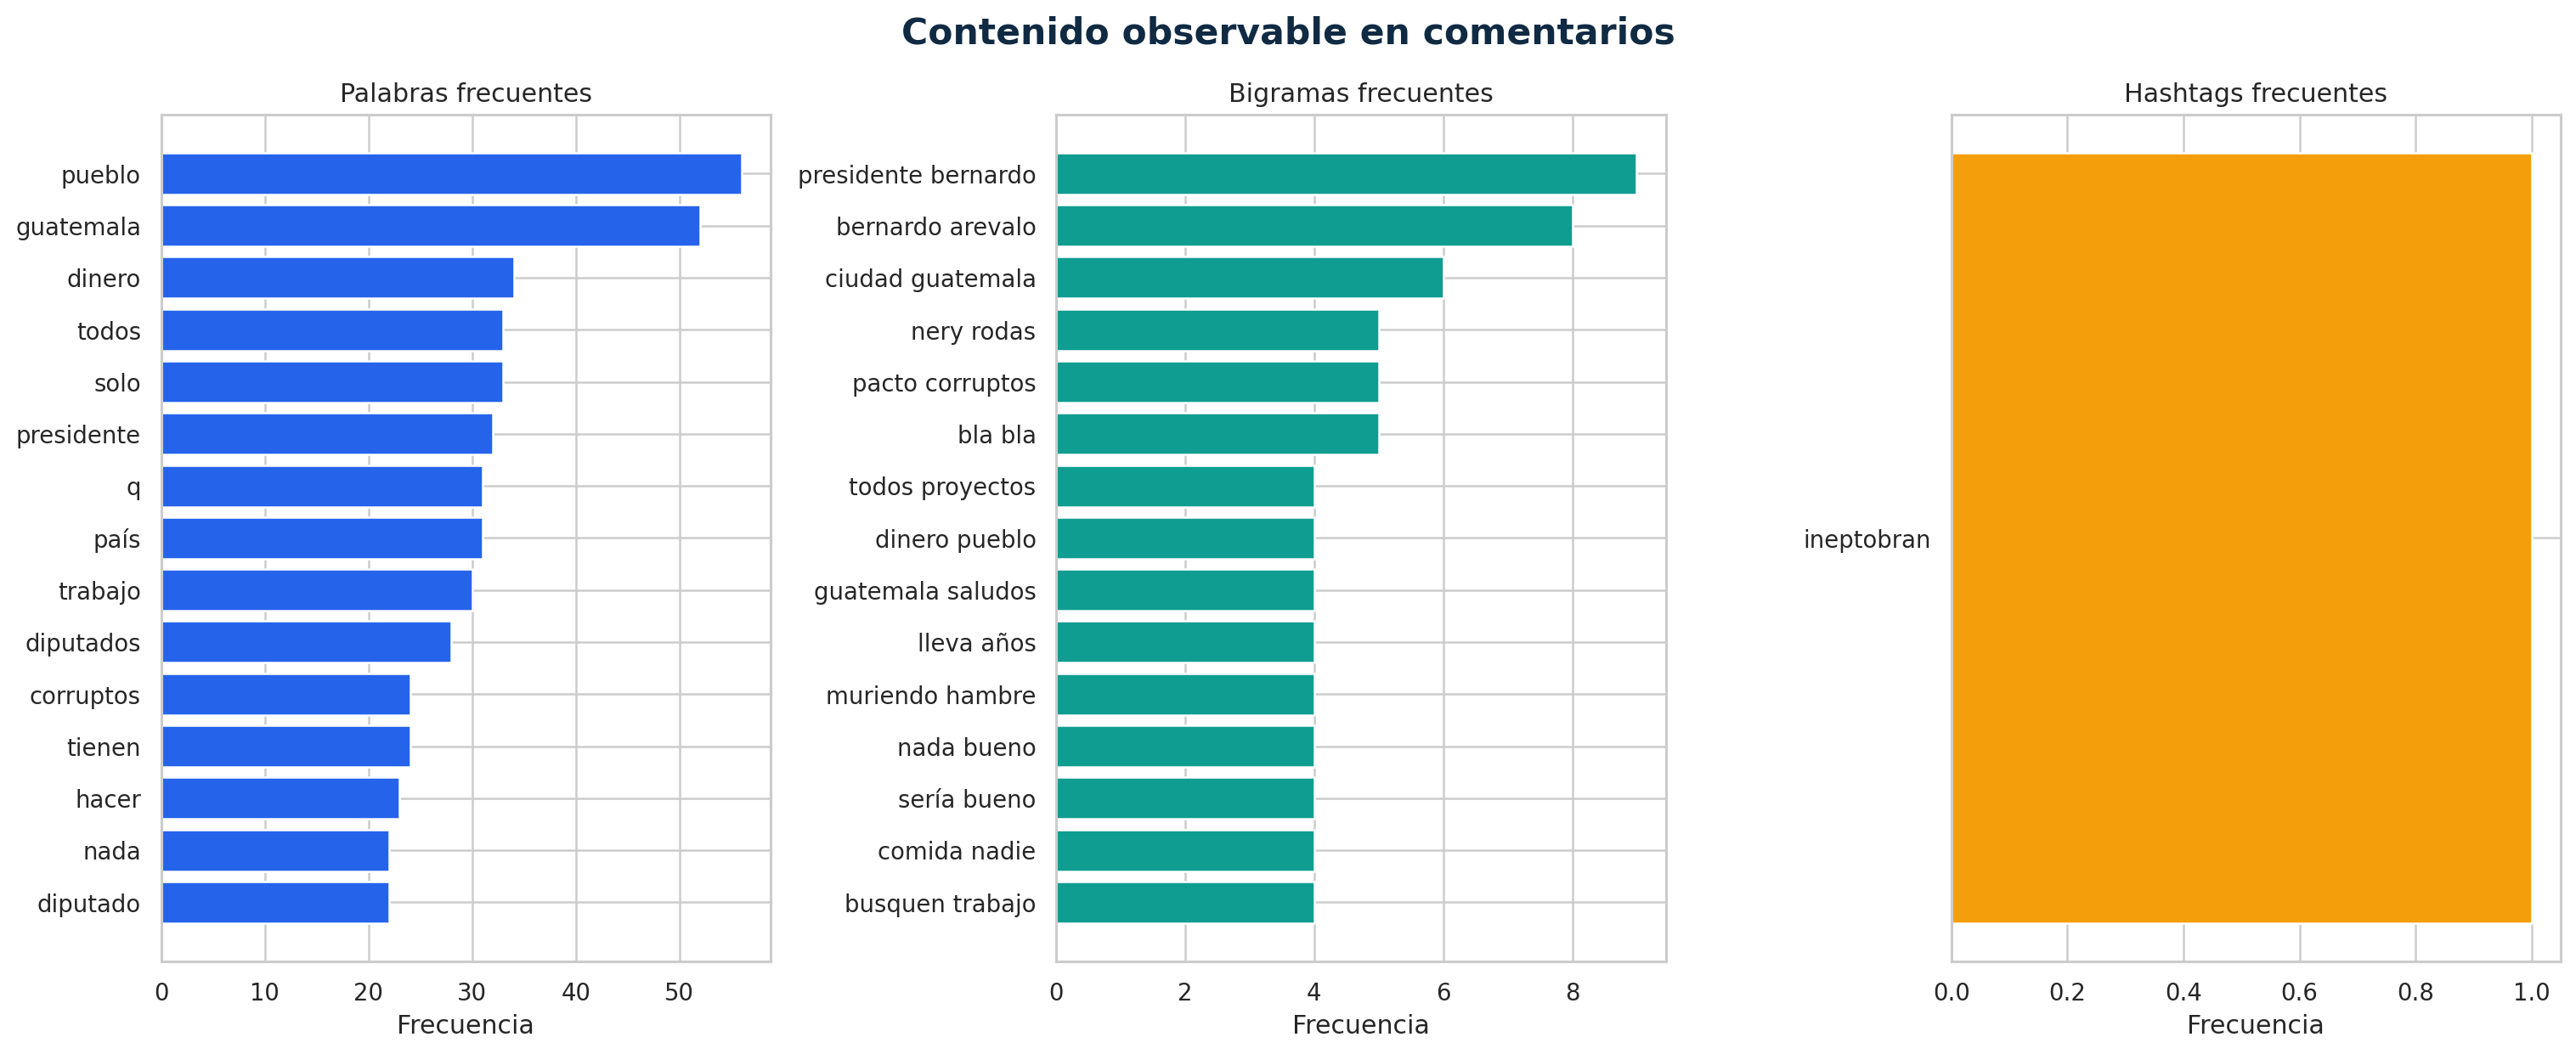
\includegraphics[width=0.98\textwidth]{frecuencias_contenido.png}
\caption{Palabras, bigramas y hashtags frecuentes después de la limpieza.}
\label{fig:texto}
\end{figure}

Las frecuencias reflejan principalmente conversación política, asuntos públicos, Guatemala, gobierno, universidad y condiciones sociales. Se reportan tanto frecuencias como probabilidades relativas en los CSV, para que los resultados sean comparables y reconstruibles. Una nube de palabras no se usó como sustituto de estas comparaciones cuantitativas.

\subsection{Concentración de participación}

\begin{figure}[H]
\centering
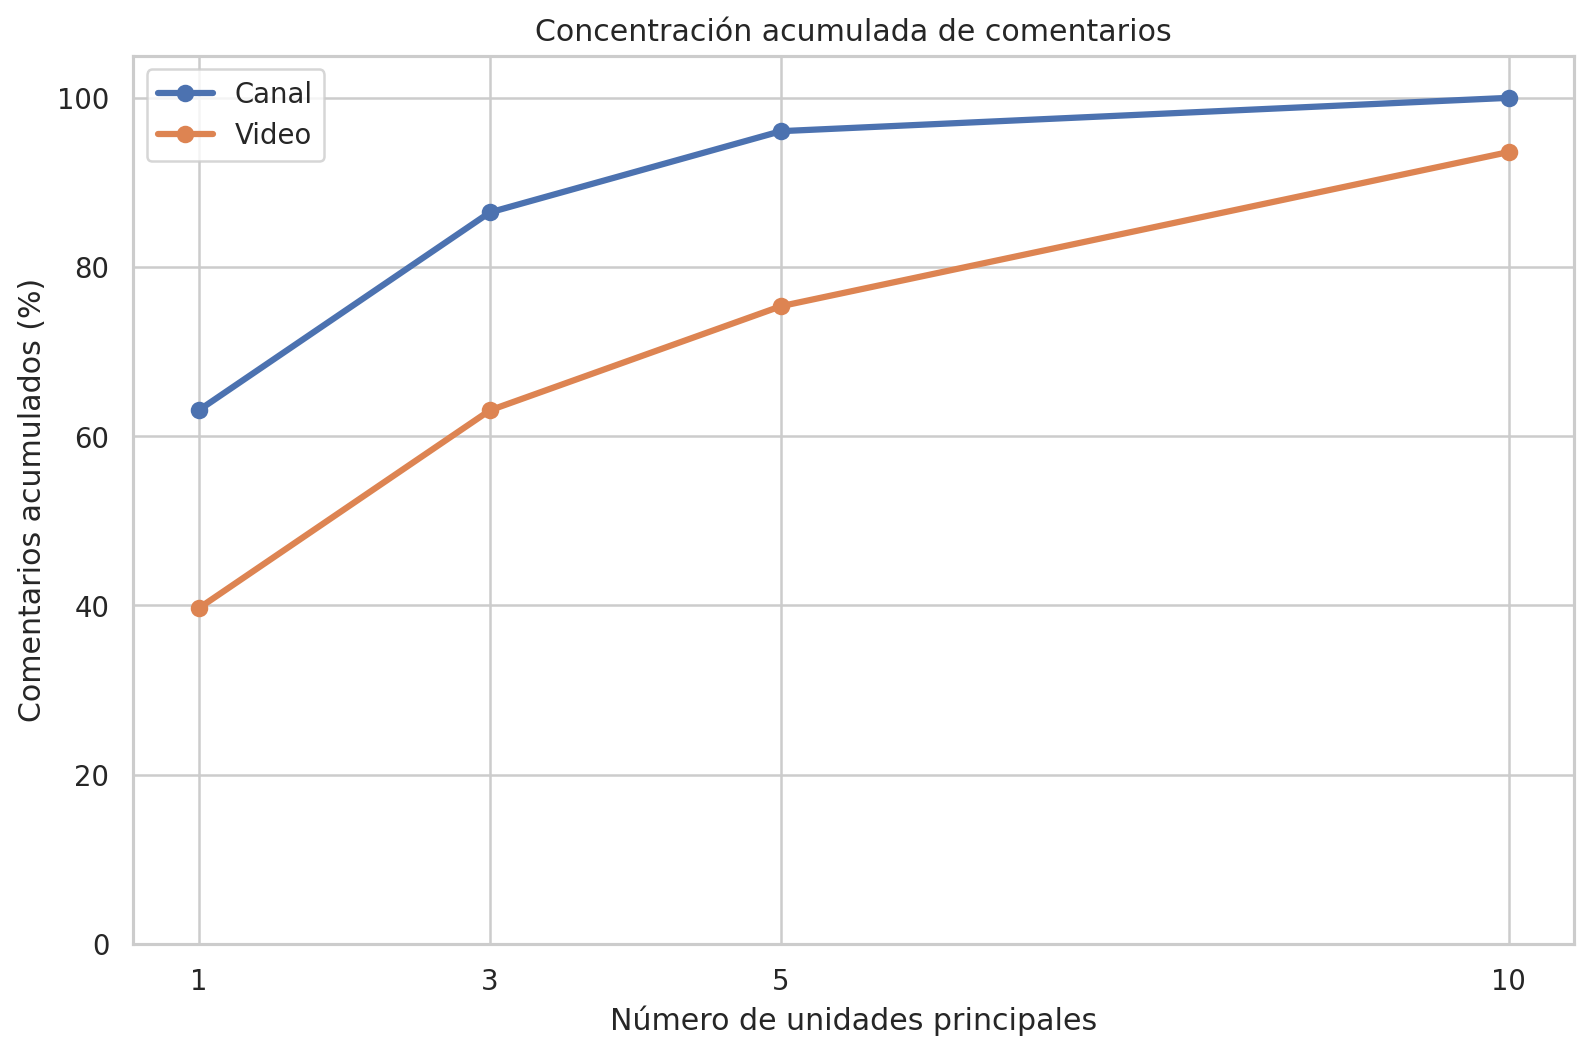
\includegraphics[width=0.78\textwidth]{concentracion_participacion.png}
\caption{Participación acumulada en las unidades más activas.}
\label{fig:concentracion}
\end{figure}

El video principal reúne 39.7\% de los comentarios; los tres primeros, 63.1\%; los cinco primeros, 75.4\%; y los diez primeros, 93.6\%. Quorum concentra 63.1\% de los comentarios, y los tres canales principales 86.5\%. Por ello, las propiedades observadas describen sobre todo unos pocos contenidos activos.

\subsection{Visibilidad y participación}

\begin{figure}[H]
\centering
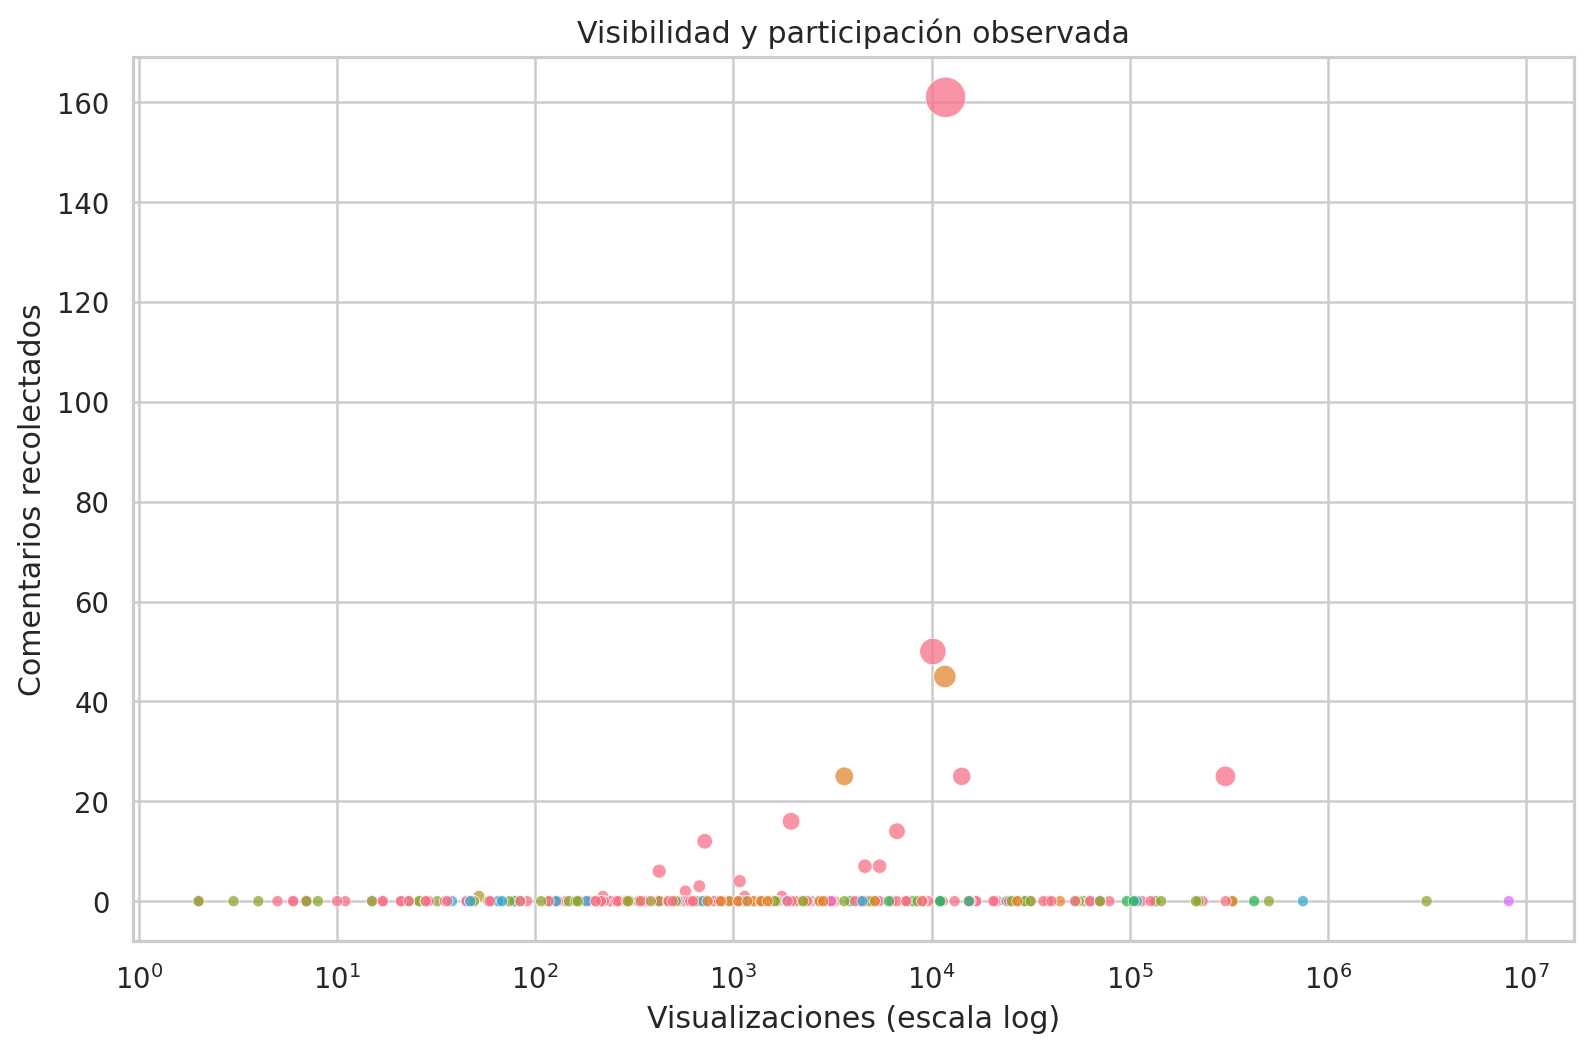
\includegraphics[width=0.78\textwidth]{visibilidad_vs_participacion.png}
\caption{Visualizaciones frente a comentarios recolectados.}
\label{fig:visibilidad}
\end{figure}

En los 293 videos, Spearman produce $\rho=0.080$ ($p=0.170$), asociación débil y no significativa. Al restringir a los 19 videos con comentarios, $\rho=0.811$ ($p<0.001$). La diferencia no debe interpretarse como contradicción: la primera estimación incorpora 274 ceros estructurales causados por cobertura, mientras la segunda sufre selección. Las visualizaciones y comentarios también fueron observados en un momento específico y no miden exactamente el mismo proceso.

\section{Preguntas obligatorias y adicionales}

\begin{enumerate}
  \item \textbf{¿Qué videos y canales concentran participación?} \emph{Qué rico come tu diputado} lidera con 161 comentarios; Quorum lidera con 256. Los cinco videos principales reúnen 75.4\%.
  \item \textbf{¿Existen audiencias compartidas?} Sí, en el sentido limitado de coparticipación: la proyección video--video contiene 11 pares unidos por autores compartidos y la proyección autor--autor 10,732 pares.
  \item \textbf{¿Qué autores funcionan como puentes?} En esta fase se identifican autores presentes en más de un video. La intermediación y el efecto de removerlos se calcularán en la fase final; anticiparlos solo con recuentos podría inducir conclusiones erróneas.
  \item \textbf{¿Qué temas y sentimientos caracterizan comunidades?} Las comunidades principales se relacionan con diputados y gasto público, gobierno y país, y USAC/corrupción. El sentimiento formal se reserva para una herramienta adecuada para español.
  \item \textbf{¿Coinciden visibilidad y participación?} No de forma general en la muestra completa: $\rho=0.080$. La asociación alta entre videos cubiertos no elimina el sesgo de selección.
  \item \textbf{¿Qué limita las conclusiones?} Consultas de búsqueda, fechas relativas, conteos instantáneos, ausencia de respuestas identificadas, 19 videos cubiertos y concentración extrema.
\end{enumerate}

Preguntas adicionales: (1) ¿qué tan recurrente es la audiencia entre videos?, respondida mediante el número de autores con más de un video; (2) ¿cuántos comentarios presentan al menos una respuesta?, sin inferir quién respondió; (3) ¿cómo se distribuye la conversación según \texttt{source\_group}?; y (4) ¿cuántos comentarios no muestran likes después de normalizar espacios? Las respuestas exactas se conservan en \texttt{preguntas\_adicionales.csv}.

\section{Red bipartita autor--video}

Se construyó una red no dirigida con autores y videos como tipos de nodo. Una arista existe cuando un autor comentó un video; su peso es el número de comentarios de ese autor en ese video. La arista no demuestra amistad, conversación directa, acuerdo ni aprobación.

\begin{figure}[H]
\centering
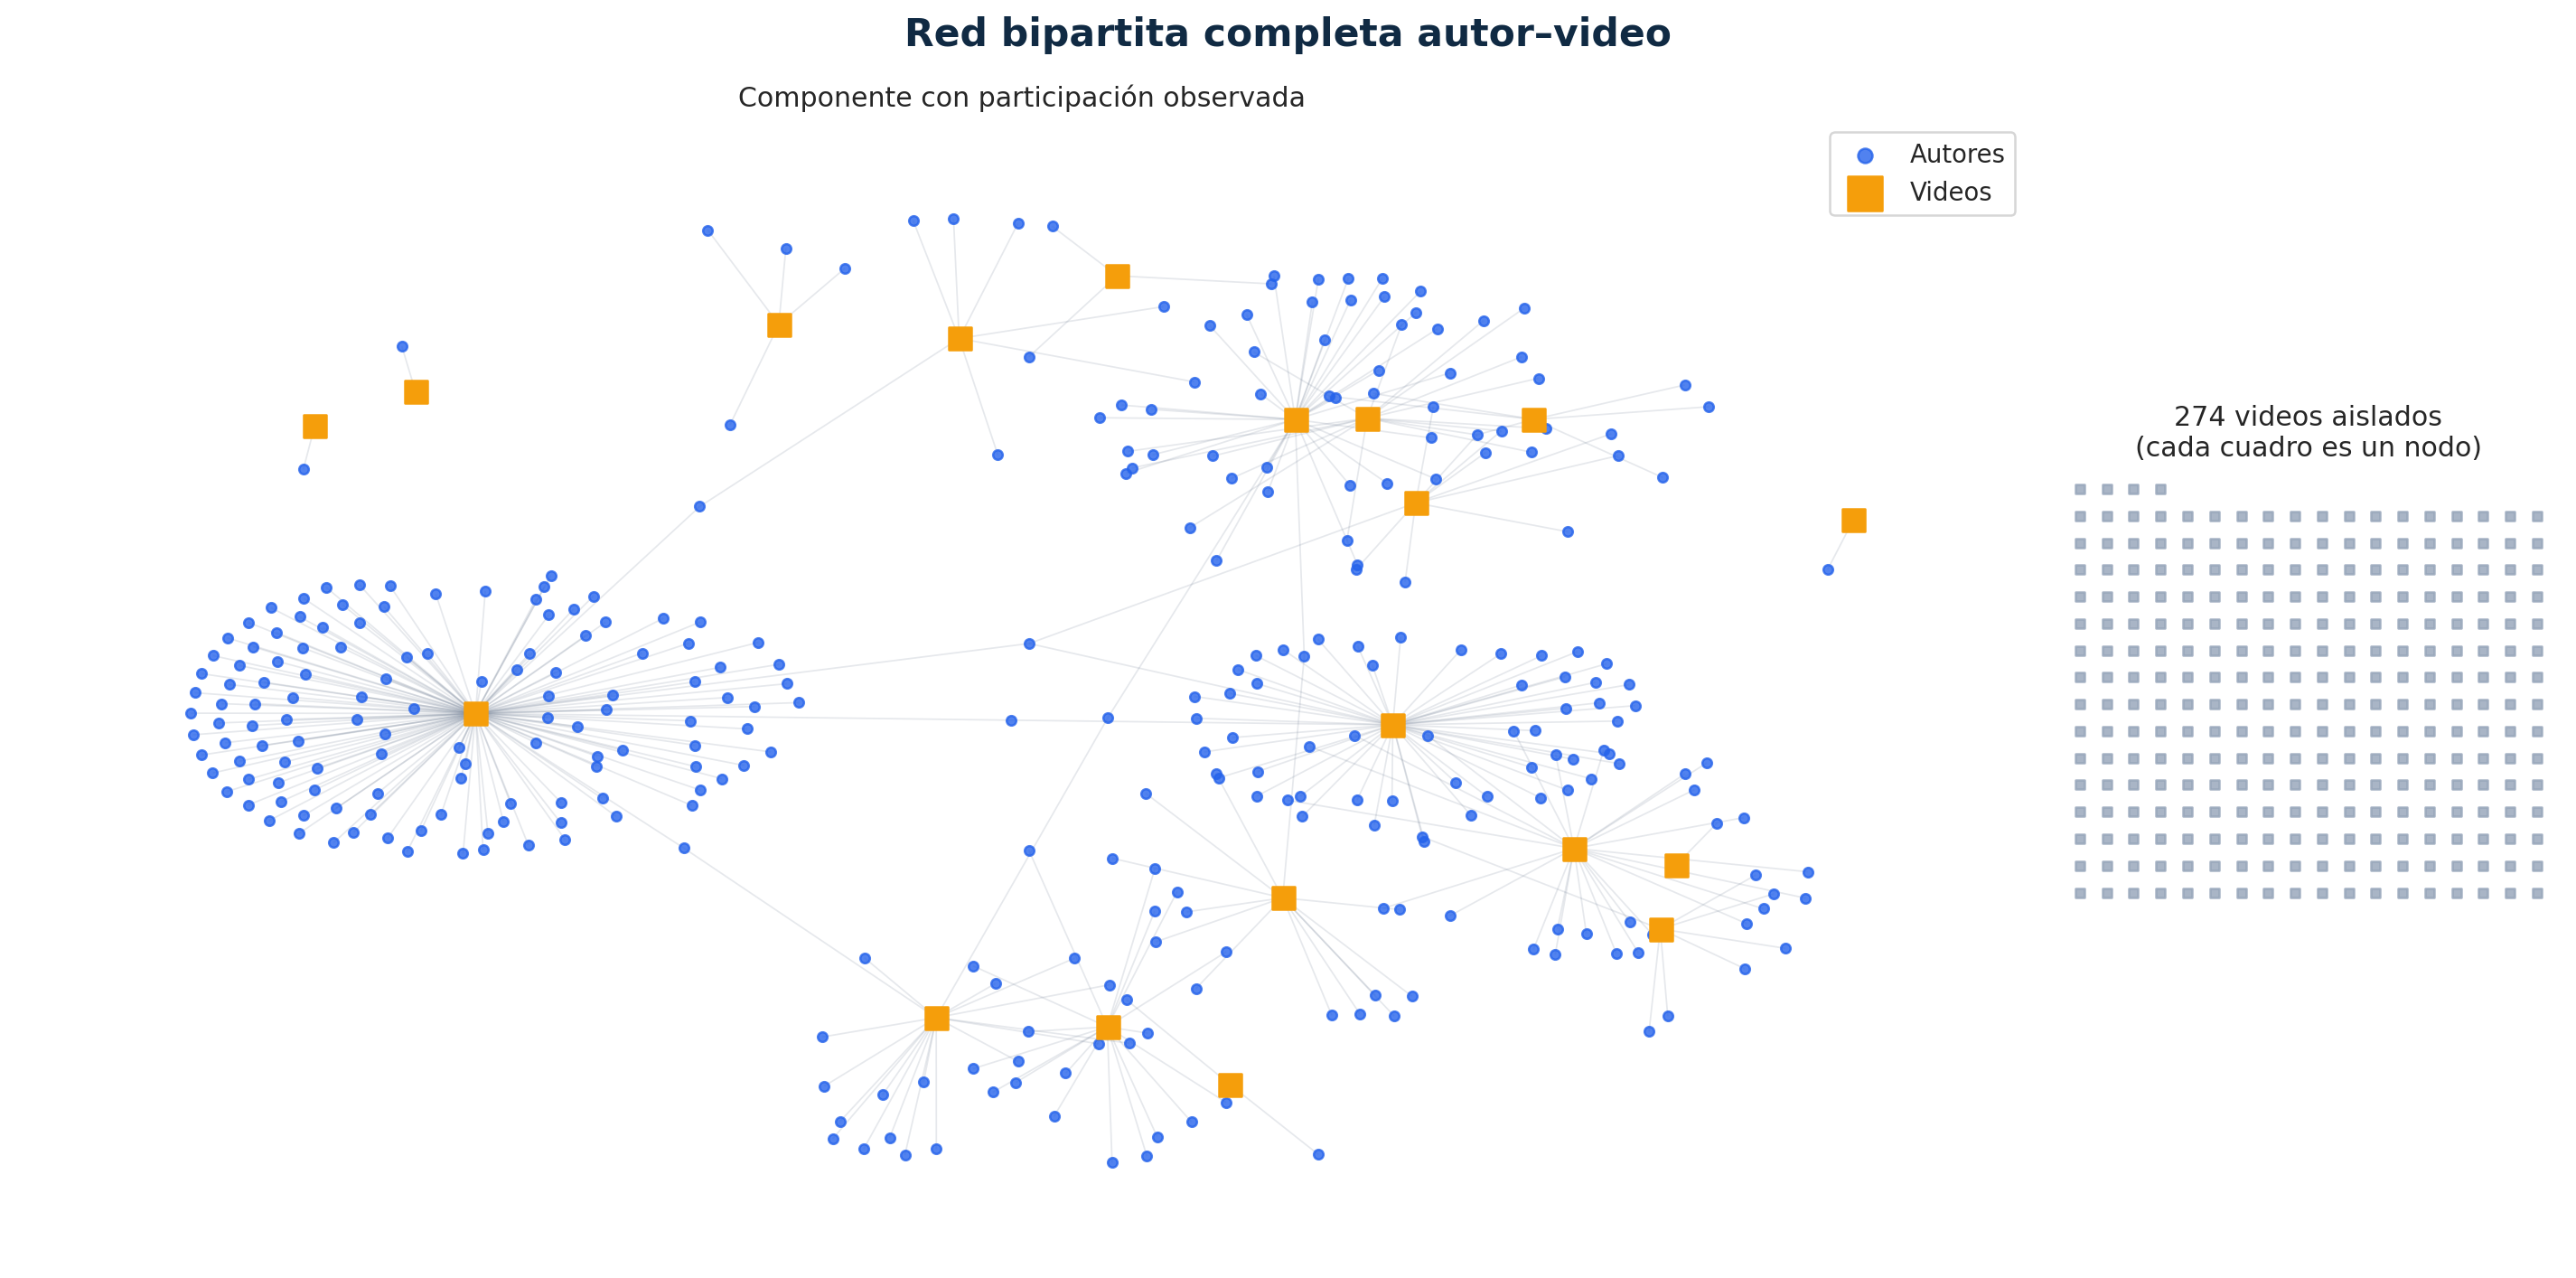
\includegraphics[width=0.98\textwidth]{red_bipartita_completa.png}
\caption{Red bipartita. La vista estructural muestra nodos activos y el panel conserva el conteo de aislados.}
\label{fig:bipartita}
\end{figure}

La tabla de nodos contiene tipo, identificador y atributos relevantes. La tabla de aristas conserva origen, destino, peso y significado. Los 274 videos sin comentarios permanecen como aislados; no se eliminaron para mejorar la apariencia.

\section{Proyecciones}

\begin{figure}[H]
\centering
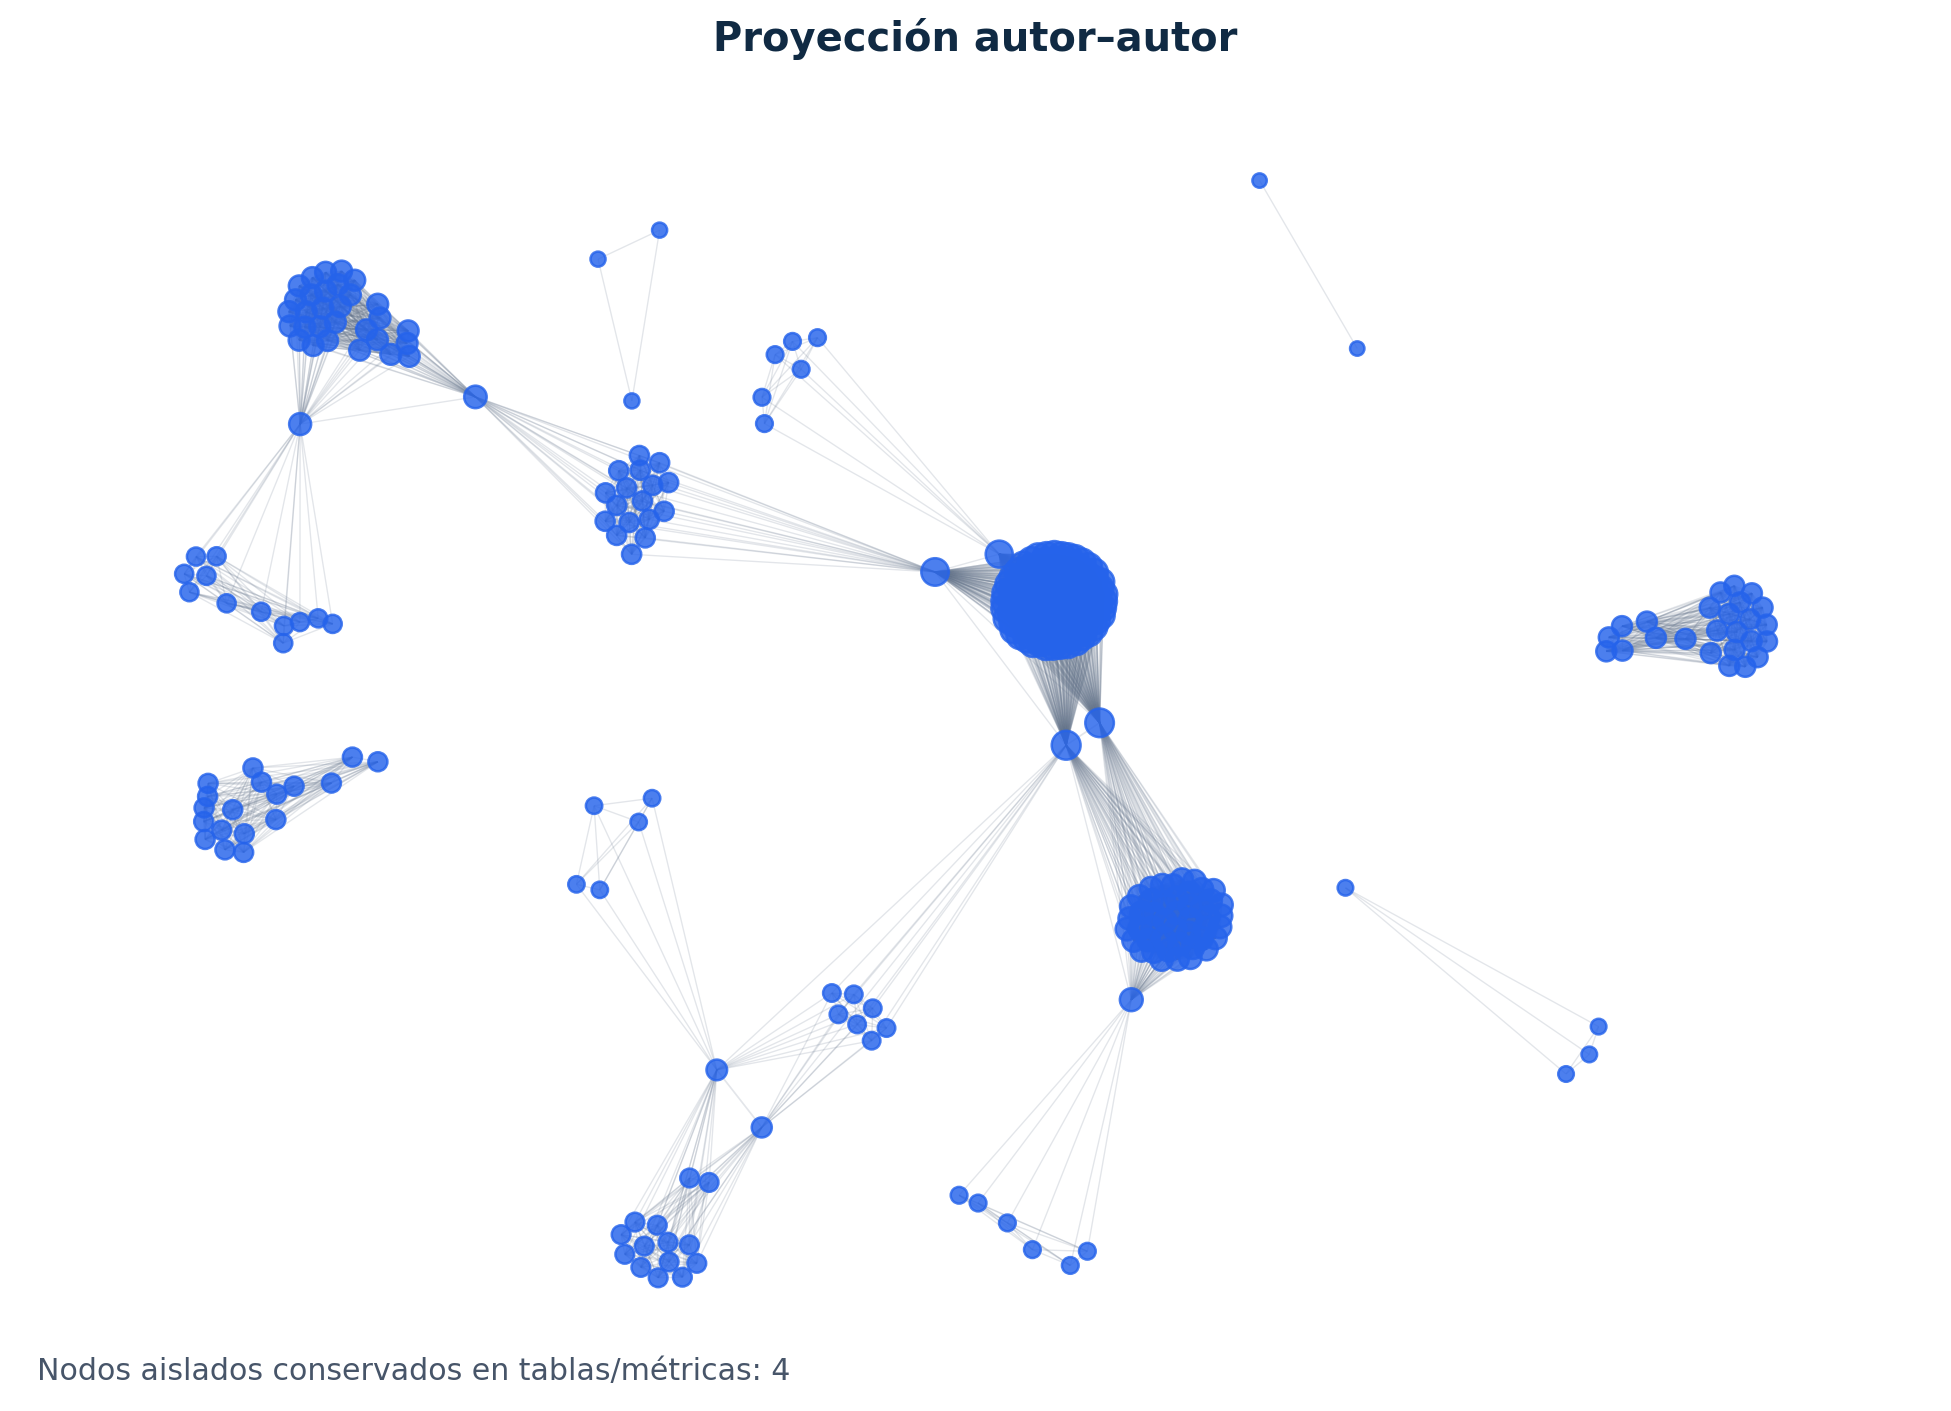
\includegraphics[width=0.82\textwidth]{proyeccion_autores.png}
\caption{Proyección autor--autor; el peso representa videos compartidos.}
\label{fig:autores}
\end{figure}

\begin{figure}[H]
\centering
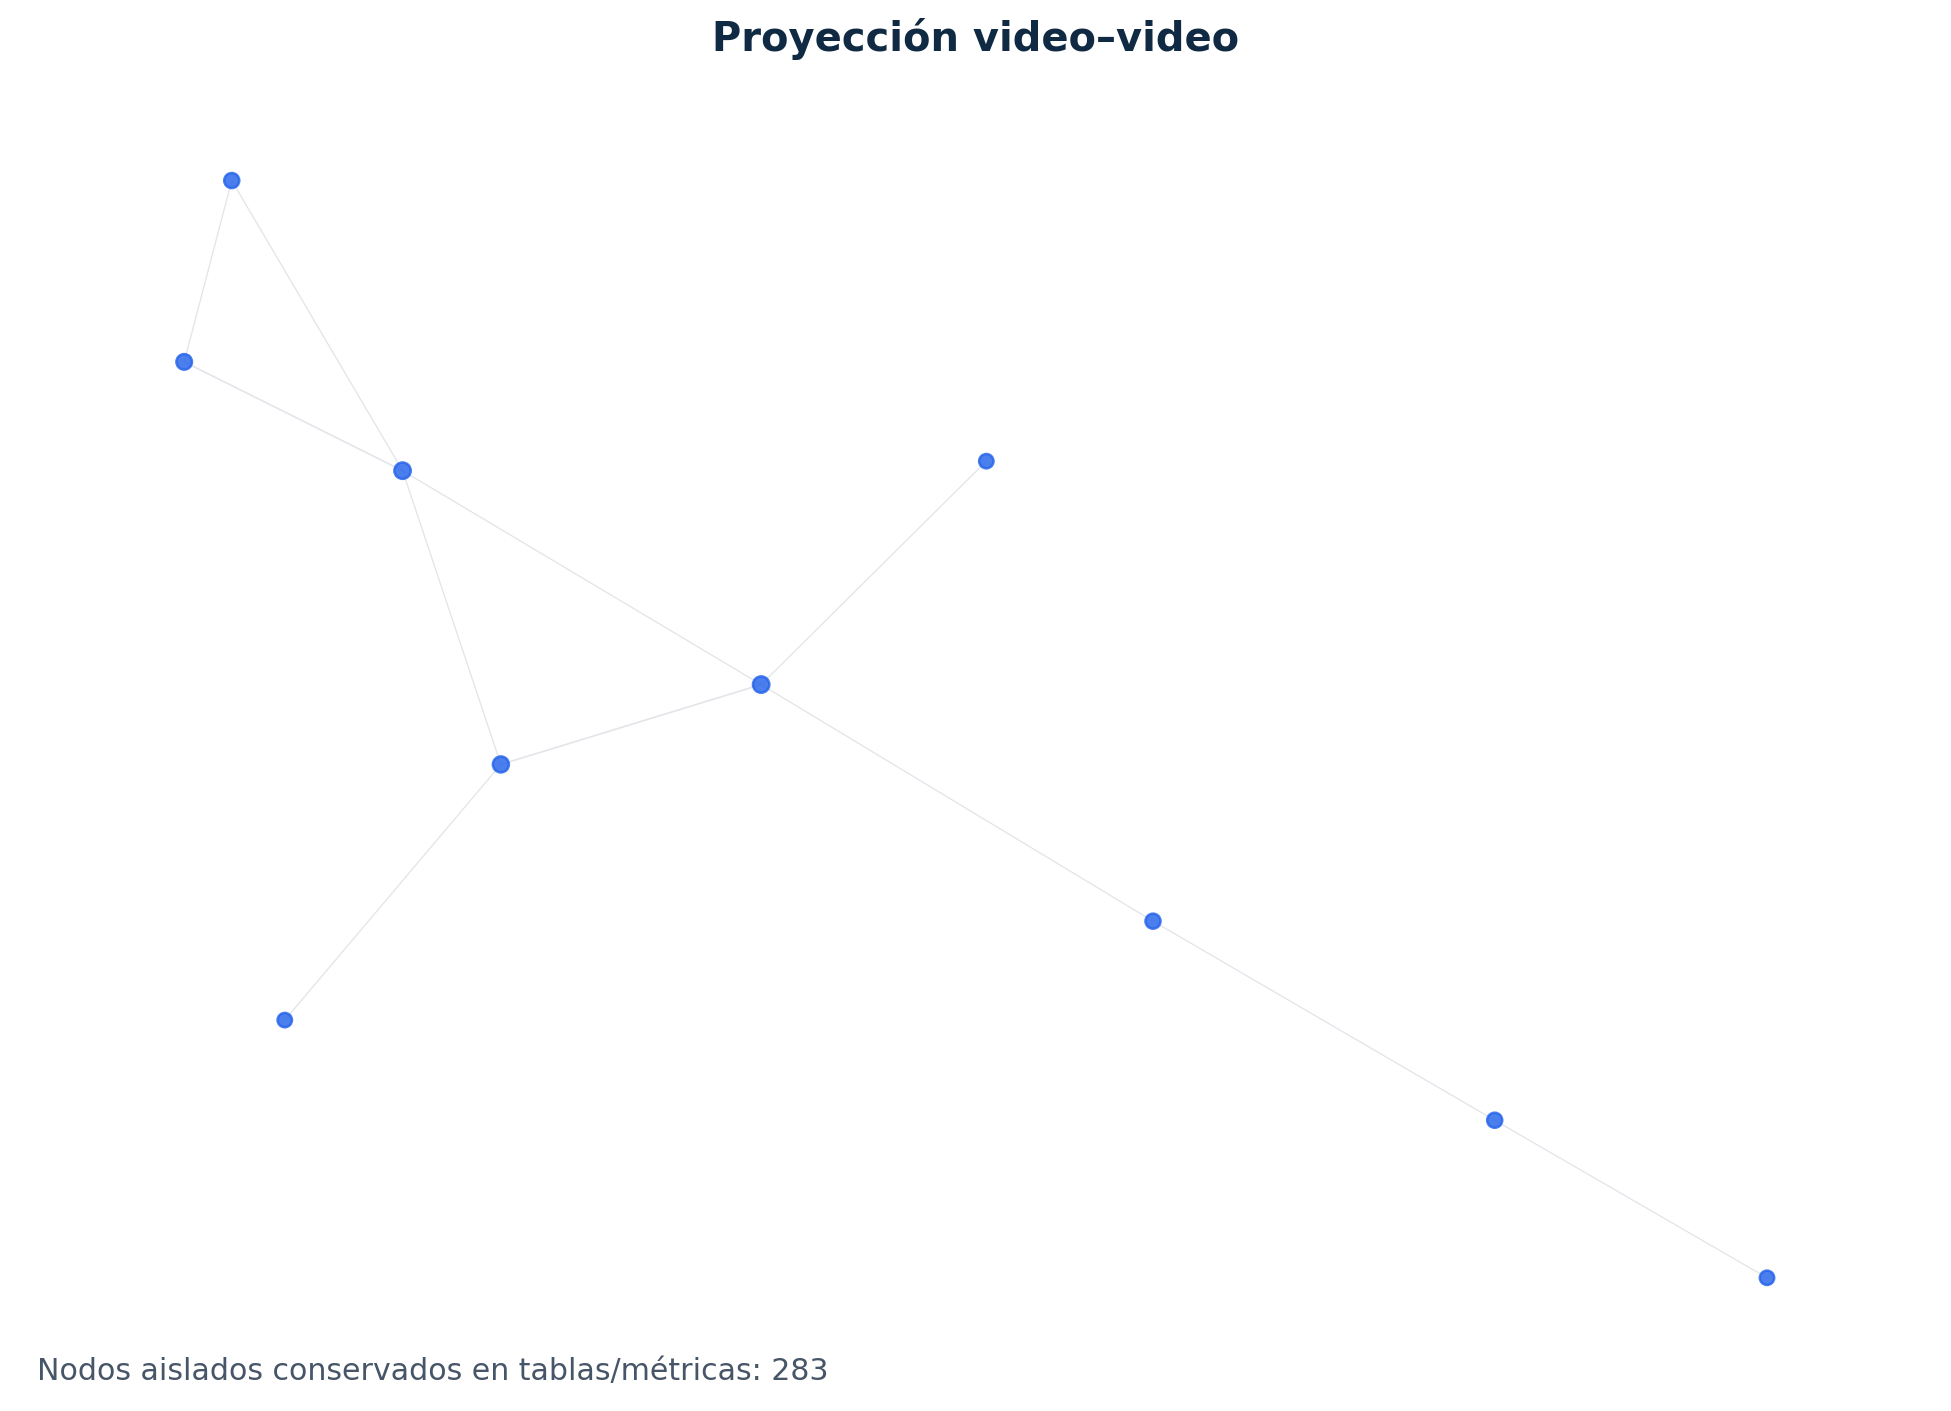
\includegraphics[width=0.82\textwidth]{proyeccion_videos.png}
\caption{Proyección video--video; el peso representa autores compartidos.}
\label{fig:videos}
\end{figure}

La proyección de autores conecta a dos cuentas cuando comentaron el mismo video; aproxima copresencia en espacios de participación, no interacción. La proyección de videos conecta contenidos que comparten al menos un autor y muestra solapamiento de audiencias. Los pesos cuentan videos o autores compartidos, respectivamente.

\section{Topología y fragmentación}

\begin{table}[H]
\centering
\caption{Métricas estructurales principales.}
\resizebox{\textwidth}{!}{%
\begin{tabular}{lrrrrrrrr}
\toprule
Red & Nodos & Aristas & Aislados & Densidad & Grado medio & Componentes & Mayor comp. & Transitividad\\
\midrule
Bipartita & 625 & 343 & 274 & 0.00176 & 1.10 & 284 & 286 & 0.000\\
Autores & 332 & 10,732 & 4 & 0.19532 & 64.65 & 10 & 276 & 0.984\\
Videos & 293 & 11 & 283 & 0.00026 & 0.08 & 284 & 10 & 0.316\\
\bottomrule
\end{tabular}}
\end{table}

\begin{figure}[H]
\centering
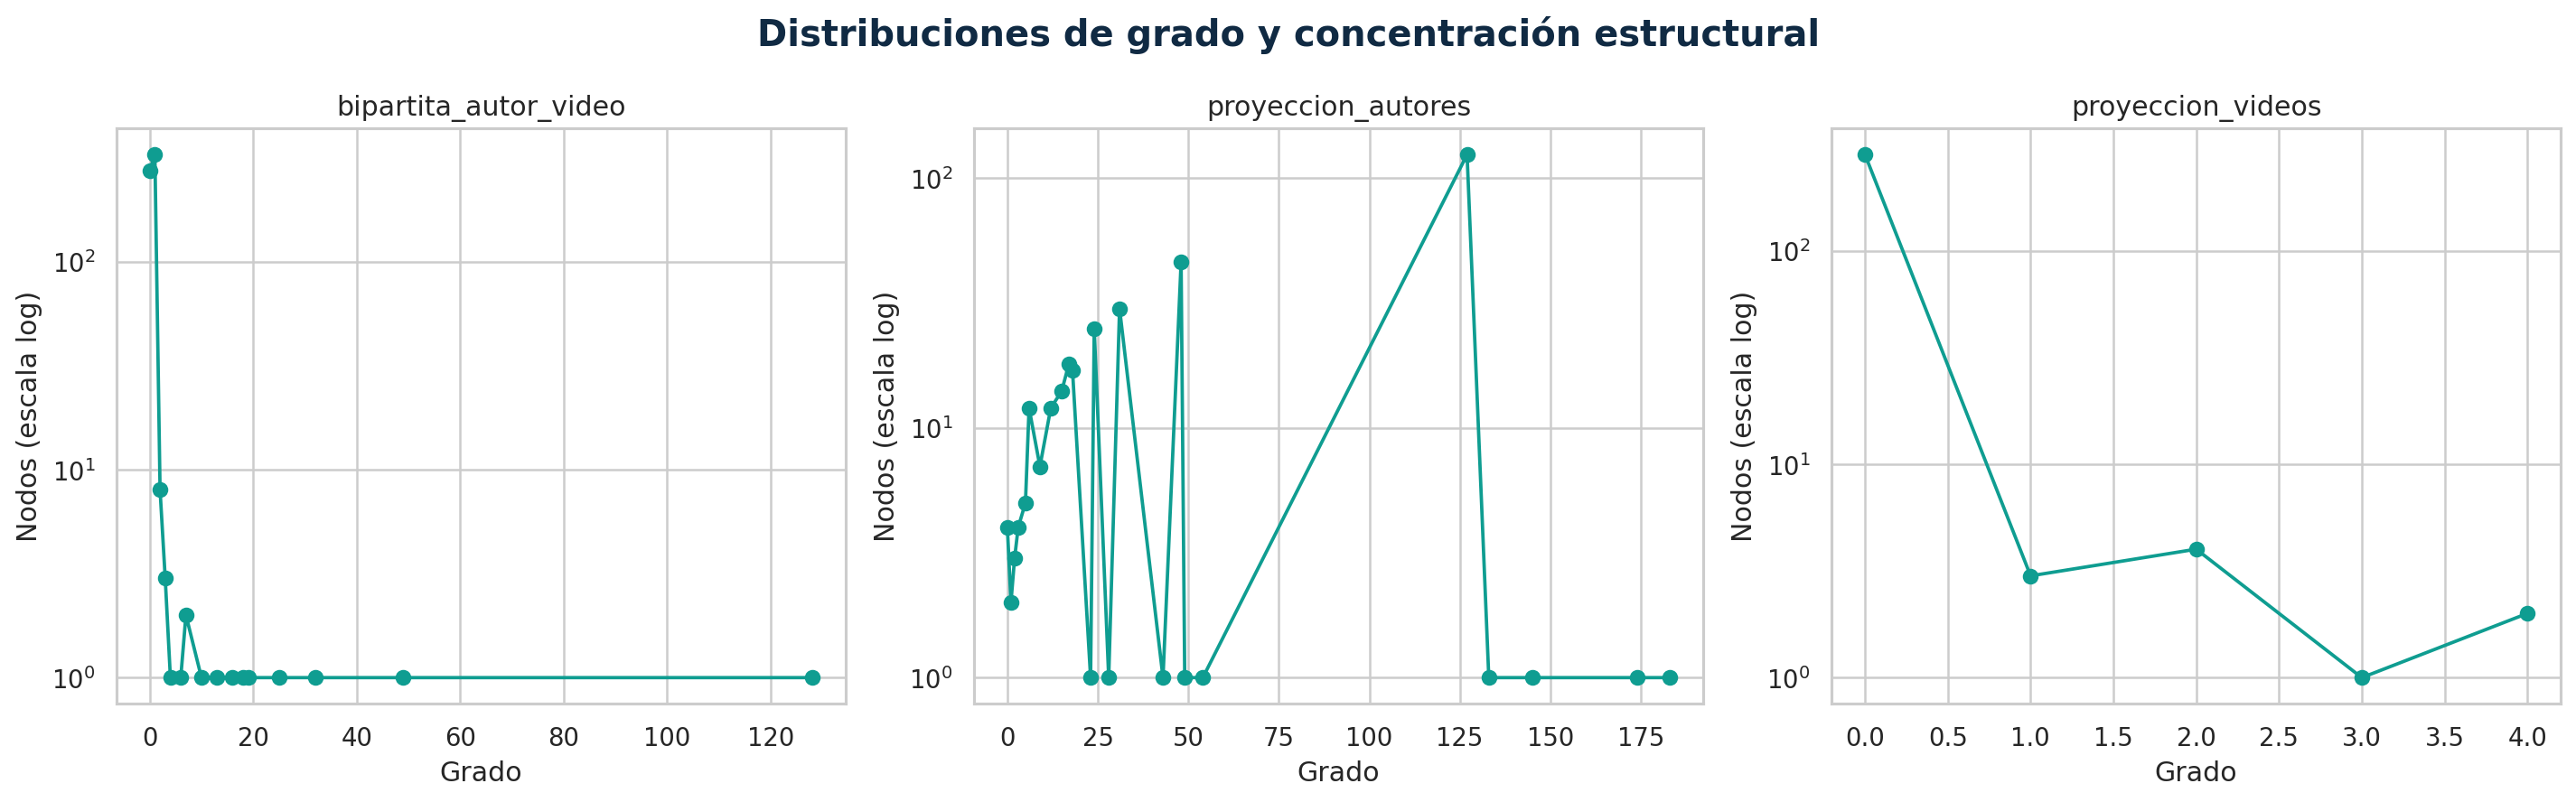
\includegraphics[width=0.98\textwidth]{distribuciones_grado.png}
\caption{Distribuciones de grado de las tres redes.}
\label{fig:grado}
\end{figure}

La red bipartita es dispersa y fragmentada por la falta de comentarios para la mayoría de videos. Su transitividad es cero por construcción: un grafo estrictamente bipartito no contiene triángulos. La proyección de autores es mucho más densa y alcanza transitividad 0.984, pero esta cifra está inflada estructuralmente porque todos los autores de un mismo video forman un clique. No representa cohesión interpersonal comprobada. La proyección de videos confirma un solapamiento muy limitado: solo diez videos tienen al menos una conexión.

La cohesión se midió en la componente conexa mayor mediante conectividad de nodos y de aristas. La conectividad de nodos es 1 en las tres redes: existe al menos un punto cuya remoción puede separar la componente. La conectividad de aristas es 1 en la bipartita y la proyección de videos, y 5 en la proyección de autores. Los diámetros de las componentes mayores también se conservan en \texttt{metricas\_redes.csv}.

Los aislados son aislamiento \emph{observado}; no prueban desinterés o inexistencia de audiencia. Pueden reflejar que no se descargaron comentarios, que la API devolvió cobertura parcial o que el procedimiento de búsqueda no capturó actividad.

\section{Comunidades}

Se eligió la proyección autor--autor porque permite estudiar conjuntos de usuarios que concurren en videos semejantes. Se aplicó Louvain ponderado con semilla 42, donde el peso es el número de videos compartidos. Los cuatro aislados de la proyección se conservaron en las métricas pero se excluyeron de la optimización de modularidad porque no aportan enlaces.

\begin{figure}[H]
\centering
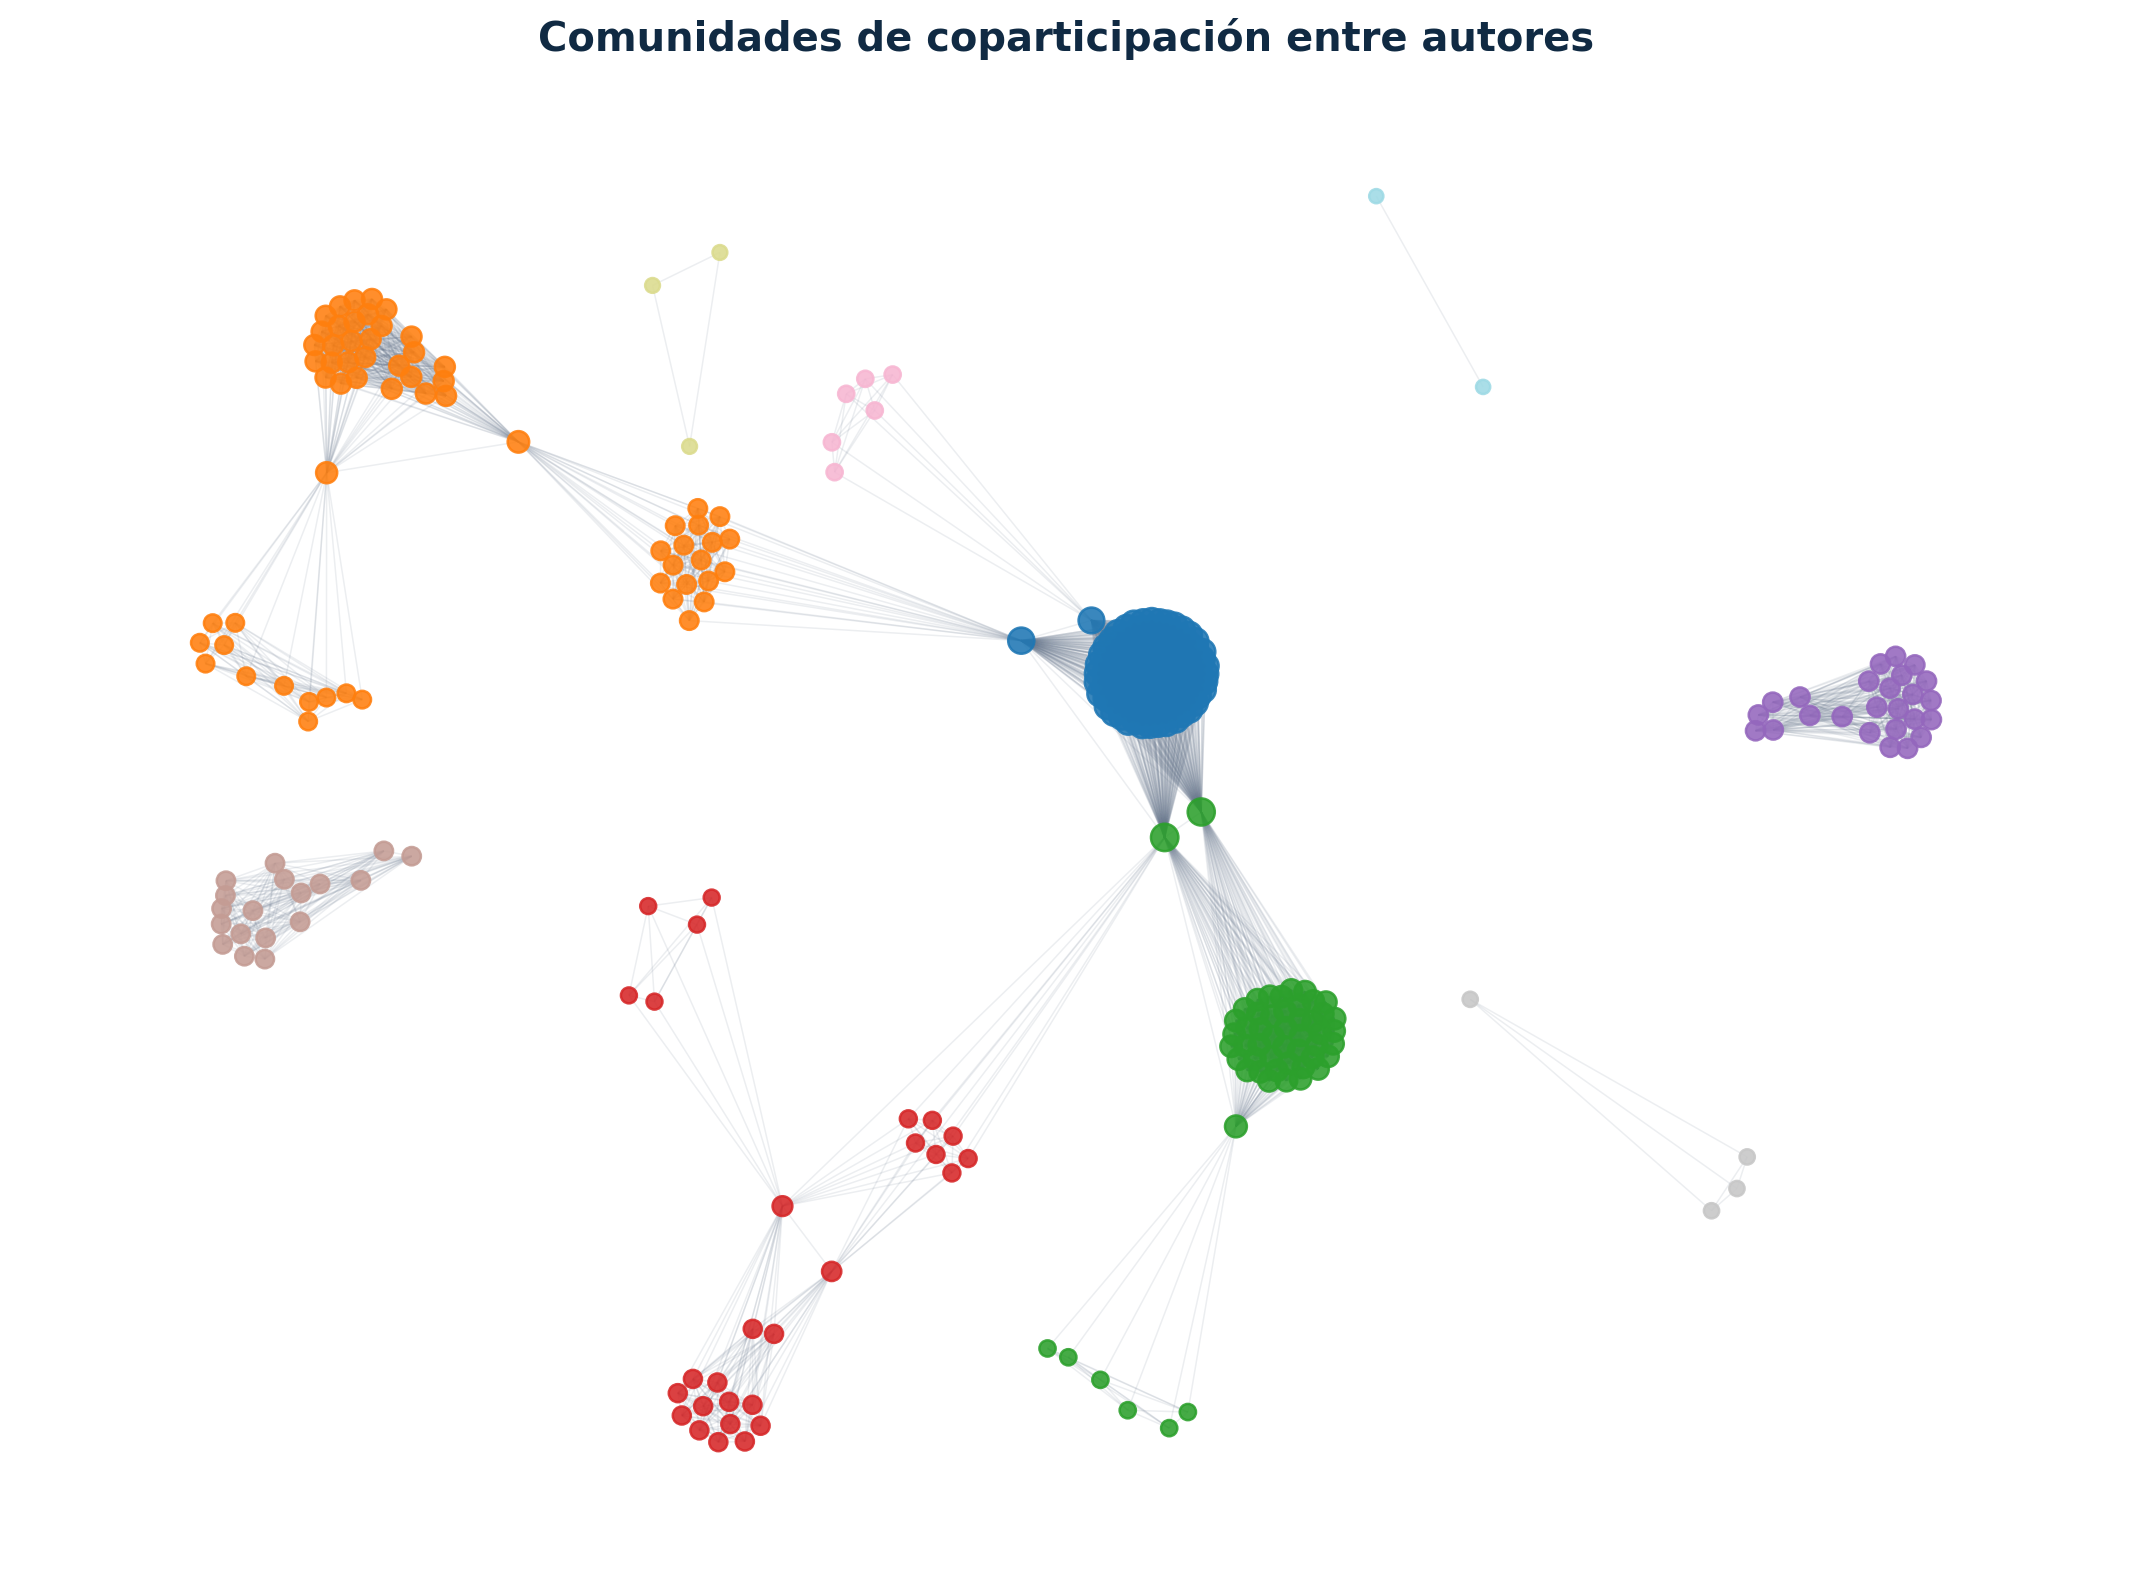
\includegraphics[width=0.88\textwidth]{comunidades_autores.png}
\caption{Diez comunidades de coparticipación detectadas mediante Louvain.}
\label{fig:comunidades}
\end{figure}

La modularidad fue 0.395. La comunidad 1 reúne 126 autores y 161 comentarios, con vocabulario sobre pueblo, dinero y diputados. La comunidad 2 contiene 61 autores y 83 comentarios relacionados con presidencia, Guatemala y gobierno. La comunidad 3 contiene 55 autores y 60 comentarios, destacando USAC, universidad y corrupción. Estas comunidades reflejan agrupación por contenidos compartidos; no son grupos sociales confirmados.

\section{Limitaciones}

\begin{itemize}
  \item Solo 19 de 293 videos tienen comentarios, de modo que 274 aislados representan principalmente cobertura desigual.
  \item La selección por consultas y canales condiciona categorías, actores y temas visibles.
  \item \texttt{published\_time} y \texttt{published\_text} son tiempos relativos y no fechas exactas.
  \item Visualizaciones, likes y respuestas son conteos observados durante la recolección y cambian con el tiempo.
  \item No existen relaciones explícitas autor--autor ni datos sobre quién respondió a quién.
  \item La alta transitividad de la proyección de autores surge en parte de la proyección de grupos que comentan un mismo video.
  \item La concentración en pocos videos impide generalizar a todos los usuarios de YouTube o a la población de Guatemala.
\end{itemize}

Se distingue descripción de asociación e inferencia: las métricas describen esta muestra; las correlaciones representan asociaciones condicionadas por recolección; no se realizan inferencias causales o poblacionales.

\section{Conclusiones preliminares}

La conversación observada se concentra en contenidos políticos y públicos de pocos canales, especialmente Quorum. La visibilidad global no coincide necesariamente con la participación recolectada, porque la mayoría de videos carece de comentarios en el archivo. La red revela una gran estructura de coparticipación entre autores, pero su densidad y transitividad deben entenderse como consecuencias de comentar videos comunes. Las comunidades muestran agrupaciones temáticas plausibles, no amistades ni coordinación demostrada.

El avance establece una base reproducible y auditable. La siguiente fase medirá centralidades y articulación, aplicará sentimiento adecuado para español, integrará esa señal en las comunidades y cerrará la interpretación conjunta.

\section{Reproducibilidad}

El flujo principal se ejecuta con \texttt{python scripts/run\_advance.py}; el notebook se reconstruye con \texttt{python scripts/build\_notebook.py}. Las tablas y figuras se generan automáticamente. El cargador acepta CSV real y libros Excel aunque la extensión sea incorrecta. La suite automatizada valida lectura, reparación de IDs, conteos, limpieza y significado de pesos. Código, dependencias e instrucciones están disponibles en \repo.

\begin{thebibliography}{9}
\bibitem{networkx} Hagberg, A., Schult, D. y Swart, P. (2008). \emph{Exploring network structure, dynamics, and function using NetworkX}. Proceedings of SciPy.
\bibitem{louvain} Blondel, V., Guillaume, J., Lambiotte, R. y Lefebvre, E. (2008). \emph{Fast unfolding of communities in large networks}. Journal of Statistical Mechanics.
\bibitem{centrality} Freeman, L. (1979). \emph{Centrality in social networks: Conceptual clarification}. Social Networks, 1(3), 215--239.
\end{thebibliography}

\end{document}
